\documentclass[fleqn]{article}

\usepackage{polski}
\usepackage[utf8]{inputenc}
\usepackage[polish]{babel}
\usepackage{parskip}
\usepackage{icomma}
\usepackage[a4paper,includeheadfoot,margin=2.54cm]{geometry}
\usepackage{svg}
\usepackage{float}
\usepackage{graphicx}
\usepackage{amsmath}
\usepackage{subcaption}

\renewcommand\thesection{\arabic{section}.}
\renewcommand\thesubsection{\arabic{section}. \alph{subsection})}
\renewcommand\thesubsubsection{}

\brokenpenalty=1000
\clubpenalty=1000
\widowpenalty=1000

\title{TM -- Laboratorium 1.}
\author{Krystian Chachuła \\ Dawid Gruszczyński \\ Marcin Skrzypkowski}

\begin{document}

\maketitle

\setcounter{page}{0}
\thispagestyle{empty}

\pagebreak

\setcounter{page}{1}

\section{Odczytywanie przebiegów instrukcji na oscyloskopie}

Lorem ipsum dolor sit amet, consectetur adipiscing elit. Pellentesque gravida, est non consectetur dapibus, mauris massa pretium tortor, ut congue ex ligula at ante. Praesent blandit risus eu quam mattis, eu vulputate ante luctus. Etiam vitae quam justo. In sit amet hendrerit velit, non feugiat enim. In sit amet porttitor justo. Orci varius natoque penatibus et magnis dis parturient montes, nascetur ridiculus mus. Suspendisse potenti. Morbi facilisis lectus venenatis mauris lacinia, in aliquet ligula semper. Ut placerat, mauris at hendrerit consequat, eros odio efficitur nisl, non fringilla lorem nisl ac diam. Donec eget egestas dui. Sed ultricies pulvinar eros, sit amet ultrices mauris efficitur ut. Donec at ligula pretium, varius diam eu, aliquet urna. Quisque condimentum, nulla iaculis pharetra cursus, purus felis posuere tellus, quis interdum ante velit vel libero. Donec eget egestas ante. In posuere odio nec libero dignissim, a mollis felis laoreet.

\begin{figure}[H]
	\centering
	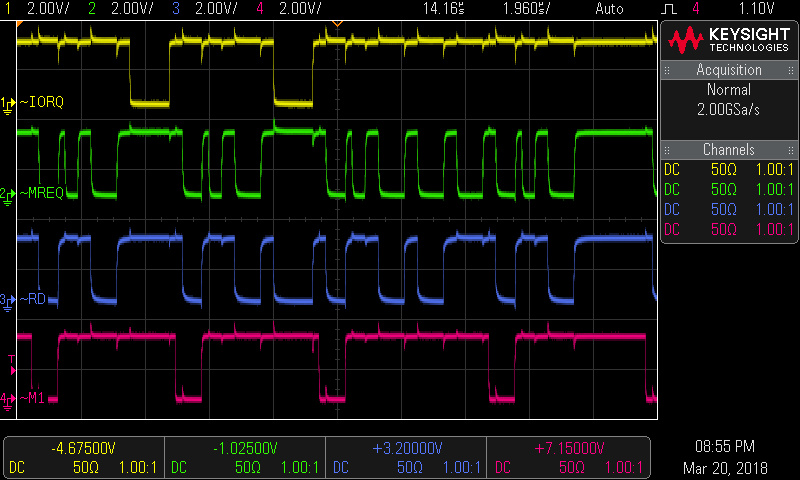
\includegraphics[width=0.75\textwidth]{img/1a.png}
	\caption{}
\end{figure}

\section{Generowanie sygnału opóźniającego}

Naszym zdaniem było wstawianie dwóch taktów opóźnienia przy odczytywaniu danych z przestrzeni wejścia/wyjścia. Procesor autoamatycznie wstawia jeden takt opóźniena przy przy wykonywaniu instrukcji dotyczących tej przestrzeni, zatem łącznie mieliśmy uzyskać trzy takty opóźniena.

Pierwszą naszą czynnościa było stworzenie funkcji logicznej, która przymowała wartość $1$, gdy był spełniony warunek z treści zadania lub $0$ w pozostałych przypadkach. Następnie zaprojektowaliśmy układ kombinacyjny realizujący tę funkcję. Początkowo wykorzystaliśmy bramki \textit{NAND} oraz \textit{NOT}, ale ze względu na trudność modyfikacji oraz małą przejrzystość takiego układu finalnie zdecydowaliśmy, że użyjemy multipleksera.

% TODO: napisać o module SML-3 z rejestrem
Do odliczania taktów zegara procesora zdecydowaliśmy się użyć rejestru przesuwnego z modułu SML-3. Pozwala on zliczyć maksymalnie 4 takty zegara, więc biorąc pod uwagę wbudowany takt oczekiwania byliśmy w stanie dodać maksymalnie 3 takty. ale było to wystarczające do wykonania zadania. Wejściem zegarowym rejestru był zanegowany sygnał zegarowy, gdyż pozwalało to uzyskać maksymalną liczbę taktów opóźnienia. Przy niezanegowanym sygnale zegarowym zawartość rejestu była przesuwana w s Alternatywą byłoby użycie licznika, lecz rejestr był rozwiązaniem prostszym.

Wyjście multipleksera oraz najmniej znaczący bit rejestru zostały doprowadzone do wejść bramki \textit{NAND}. W ten sposób otrzymaliśmy wymagany sygnał $\overline{WAIT}$.

\begin{figure}[H]
	\centering
	\begin{subfigure}[b]{0.49\textwidth}
		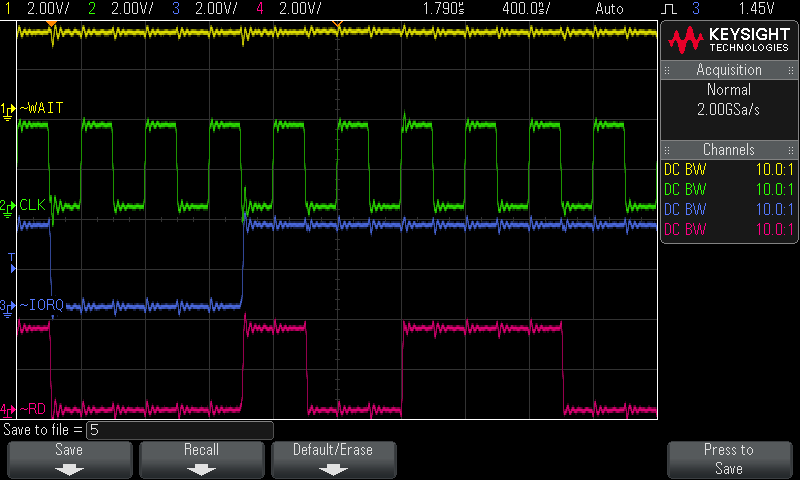
\includegraphics[width=\textwidth]{img/2a.png}
		\caption{}
	\end{subfigure}
	\begin{subfigure}[b]{0.49\textwidth}
		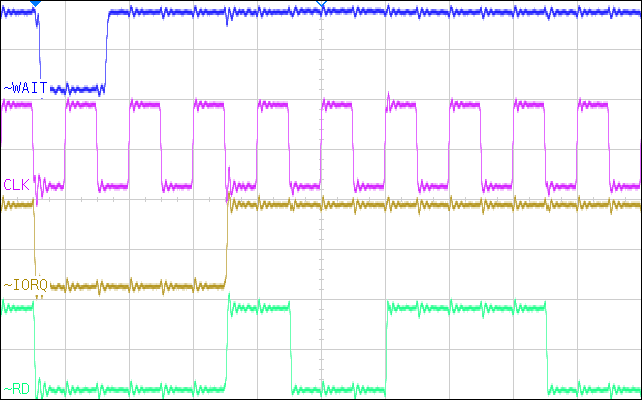
\includegraphics[width=\textwidth]{img/2b.png}
		\caption{}
	\end{subfigure}
	\begin{subfigure}[b]{0.49\textwidth}
		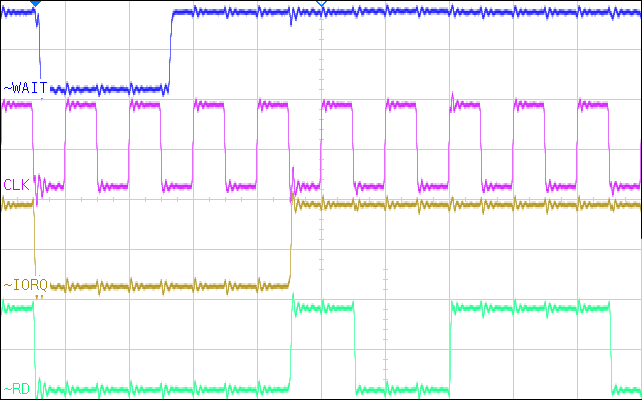
\includegraphics[width=\textwidth]{img/2c.png}
		\caption{}
	\end{subfigure}
	\begin{subfigure}[b]{0.49\textwidth}
		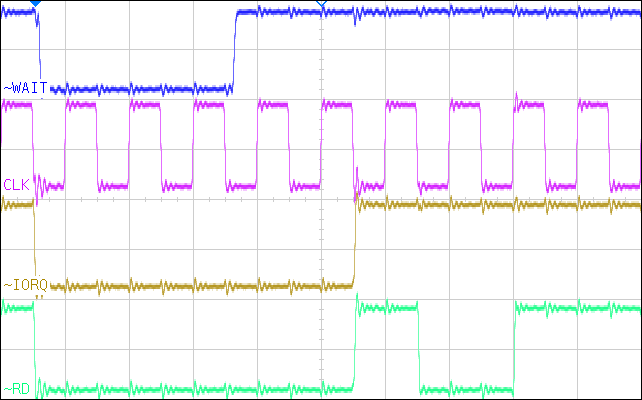
\includegraphics[width=\textwidth]{img/2d.png}
		\caption{}
	\end{subfigure}
	\begin{subfigure}[b]{0.49\textwidth}
		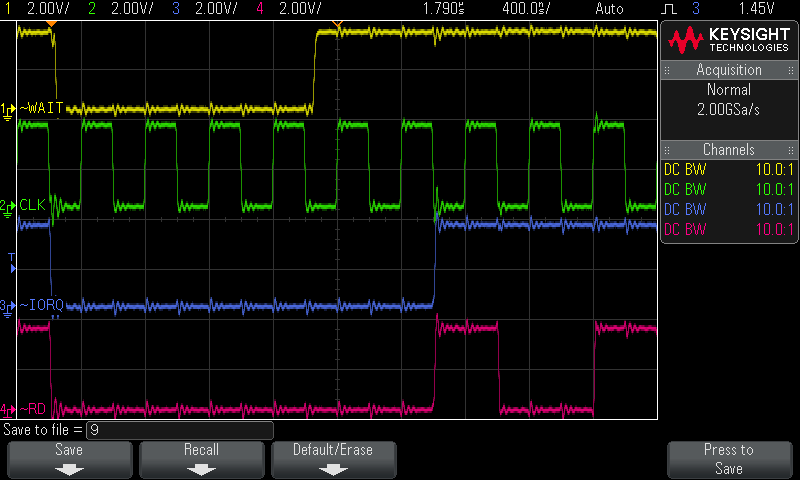
\includegraphics[width=\textwidth]{img/2e.png}
		\caption{}
	\end{subfigure}
	\caption{}
\end{figure}

\section{Wstrzymywanie pracy procesora}

\begin{figure}[H]
	\centering
	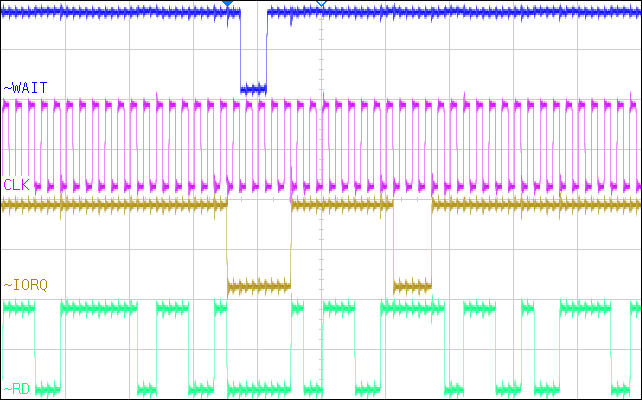
\includegraphics[width=0.75\textwidth]{img/3a.png}
	\caption{}
\end{figure}

\begin{figure}[H]
	\centering
	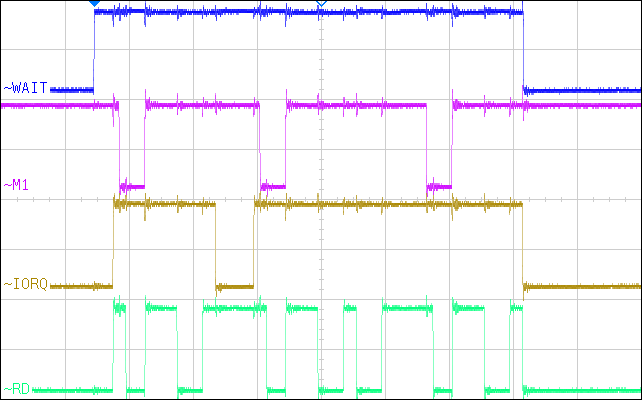
\includegraphics[width=0.75\textwidth]{img/3b.png}
	\caption{}
\end{figure}

\begin{figure}[H]
	\centering
	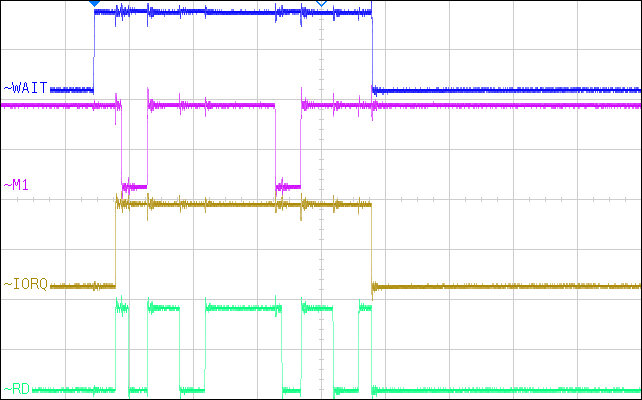
\includegraphics[width=0.75\textwidth]{img/3c.png}
	\caption{}
\end{figure}

\end{document}
